\chapter{Introduction}\label{ch:introduction}

% Goals:
% - contextualize RC in physics
% - new field, interest, ML physics
% - outline rest, put important figures in intro
% - who helped and what did I do

Recently, many difficult problems have been solved using methods from
the field of machine learning, in particular using neural
networks. Machine learning methods work by learning solutions from
example data alone, without the need for an existing model for that
data.  Physicists have used neural networks to find the masses of
particles from decay data~\cite{lonnblad1992} and separate quark and
gluon jets in $e^+ e^-$ annihilation~\cite{csabai1991}.  In other
fields, this approach has been used effectively on handwritten digit
recognition~\cite{lecun1998,simard2003}, speech
recognition~\cite{hinton2012}, and speech production~\cite{oord2016}.
These are all problems with large sets of example data, but which are
otherwise difficult or intractable with a more traditional programming
approach. Put simply, it is easy to provide examples of what the
number ``\num{2}'' looks like, while it is difficult to define what
features a written ``\num{2}'' must have in a programming language.

By its nature, many problems in physics are defined in terms of
time-varying data. Neural networks that contain internal cycles,
called recurrent neural networks, are a natural fit for these
problems. The addition of cycles gives the resulting network memory
and allows it to be used to effectively solve many time-domain
problems, such as forecasting chaotic
systems~\cite{garcia-pedrero2010}. However, this modification has a
cost: recurrent neural networks take much more time to train, as the
training algorithm takes exponentially longer to learn how to utilize
past inputs~\cite{bengio1994,lukosevicius2009}.

More recently, a new machine learning tool has emerged for dealing
with time-domain problems.  Known as \emph{reservoir computing}, this
tool was originally formulated as a novel way to reduce the
computational cost of training recurrent neural
networks~\cite{lukosevicius2009}. Reservoir computers (RCs) have been
effectively applied to chaotic system
forecasting~\cite{jaeger1978,pathak2017}, system state
inference~\cite{lu2017}. More than just short-term prediction, RCs are
capable of reproducing the \emph{climate} of a dynamical
system;~\cite{pathak2017,haluszczynski2019} it learns the long-term
features of the system, such as the system's attractor and Lyapunov
exponents.

RCs are interesting to physicists not only as a tool to solve
problems. At the heart of a RC is a dynamic system called the
\emph{reservoir}, which provides the rich dynamics the RC draws on to
function. This is usually implemented as a neural network, but in
practice many dynamic systems function well. This opens the door to
building RCs around real physical systems, such as a network of
autonomous logic on an FPGA~\cite{canaday2018} or an optical feedback
system~\cite{antonik2016}. This is interesting from a theoretical
perspective, as physical RCs use an ancillary system to help answer
questions about a main system, but they are also practically
interesting: by relying on physical reservoirs, rather than simulated,
these methods perform chaotic system forecasting at a very high rate.

As a new field, reservoir computing still has many unanswered
fundamental questions. What qualities should the internal reservoir
have to create a good RC? A common practice is to use a random network
as the reservoir, generated from a set of metaparameters. There are a
handful of results for some parameters, such as setting the
\emph{spectral radius} of the network near unity and the need for
recurrent network connections,\cite{jaeger2001,lukosevicius2012} but
the applicability of these results is narrow. What features of the
reservoir are necessary, and which can be discarded?

In this thesis, I will construct reservoir computers that do not
follow the conventional rules for reservoir construction. These RCs
continue to perform well on chaotic system forecasting and state
inference, and can even reproduce the chaotic attractor of the system
they have learned, despite the fact that their internal reservoir has
no recurrent connections. Indeed, by the end of this thesis, they do
not have an internal reservoir at all.

\section{Outline and Summary of Contributions}

%\begin{reusefigure}{fig:reservoir}
%  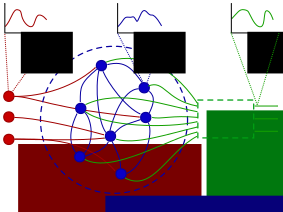
\includegraphics[width=0.6\textwidth]{figures/reservoir}
%  \caption{Re-used caption.}
%\end{reusefigure}

In \cref{ch:reservoir-computing}, I describe the reservoir computing
method, as well as a common concrete implementation of a RC called an
echo state network (ESN). I explain how to construct an ESN, the
metaparameters that govern its construction, and discuss some of the
limited known results for choosing these metaparameters. Then, I
discuss how the RC is trained, both for autonomous forecasting tasks
and for inference tasks, as well as how performance quality on these
tasks is commonly measured. I briefly discuss the known problems with
this performance measure, and suggest a few alternative methods.

In \cref{ch:low-connectivity}, I apply RCs to the task of chaotic
system forecasting for three different chaotic systems. I use a
Bayesian optimization algorithm to tune the metaparameters for the
RCs, and in so doing, discover a class of well-performing RCs with very
simple internal reservoirs. I identify four classes of reservoir
networks with simple structure. Two of these classes had been
previously identified. I build on this work and demonstrate that all
four classes have the capacity to perform as well as a traditional
RC. In particular, all four classes can reproduce the chaotic
attractor of the system they are trained on. I then discuss the
trade-offs between these simpler reservoir structures and a
traditional RC.

In \cref{ch:nvar} I describe a different technique known as
non-linear vector autoregression (NVAR), which has recently been shown
to be mathematically equivalent to an RC under certain conditions. I
discuss the construction and training of an NVAR, and how to apply it
to common RC tasks. Then, I discuss the parallells between the NVAR
and RC approaches, as well as when the equivalence is known to
hold. Finally, I discuss the tradeoffs between the two approaches.

In \cref{ch:nvar-application}, I build on this equivalence with my
collaborators to demonstrate NVARs solving two common RC tasks: system
forecasting and state inference. I show that NVARs are capable of
RC-equivalent performance on these tasks despite being considerably
simpler than an RC, and can achieve this performance with very little
training data and training time. In addition, I discuss how a trained
NVAR can provide interpretable results, while a trained RC is
opaque. I discuss how to move beyond the strict proven mathematical
equivalence to solve a wider variety of problems, and then demonstrate
this by performing chaotic system forecasting on a system without a
known equivalence.

%In \cref{ch:nvar-hardware}, I utilize the simplicity of the NVAR
%approach to implement it in hardware on an FPGA.
% FIXME you haven't done this yet

Finally, in \cref{ch:conclusion}, I summarize my findings and
contributions, and propose interesting new directions for future
research discovered during this work.
